\documentclass[brazil]{beamer}

\mode<presentation> {

% The Beamer class comes with a number of default slide themes
% which change the colors and layouts of slides. Below this is a list
% of all the themes, uncomment each in turn to see what they look like.

%\usetheme{default}
% \usetheme{AnnArbor}
% \usetheme{Antibes}
% \usetheme{Bergen}
% \usetheme{Berkeley}
% \usetheme{Berlin}
% \usetheme{Boadilla}
% \usetheme{CambridgeUS}
% \usetheme{Copenhagen}
% \usetheme{Darmstadt}
% \usetheme{Dresden}
% \usetheme{Frankfurt}
% \usetheme{Goettingen}
% \usetheme{Hannover}
% \usetheme{Ilmenau}
% \usetheme{JuanLesPins}
% \usetheme{Luebeck}
% \usetheme{Madrid}
% \usetheme{Malmoe}
%\usetheme{Marburg}
%\usetheme{Montpellier}
%\usetheme{PaloAlto}
%\usetheme{Pittsburgh}
\usetheme{Rochester}
% \usetheme{Singapore}
% \usetheme{Szeged}
% \usetheme{Warsaw}

% As well as themes, the Beamer class has a number of color themes
% for any slide theme. Uncomment each of these in turn to see how it
% changes the colors of your current slide theme.

%\usecolortheme{albatross}
%\usecolortheme{beaver}
%\usecolortheme{beetle}
%\usecolortheme{crane}
%\usecolortheme{dolphin}
%\usecolortheme{dove}
%\usecolortheme{fly}
%\usecolortheme{lily}
%\usecolortheme{orchid}
%\usecolortheme{rose}
%\usecolortheme{seagull}
%\usecolortheme{seahorse}
%\usecolortheme{whale}
%\usecolortheme{wolverine}

%\setbeamertemplate{footline} % To remove the footer line in all slides uncomment this line
%\setbeamertemplate{footline}[page number] % To replace the footer line in all slides with a simple slide count uncomment this line

%\setbeamertemplate{navigation symbols}{} % To remove the navigation symbols from the bottom of all slides uncomment this line
}

%encoding
%--------------------------------------
\usepackage[T1]{fontenc} % codificação da fonte em 8-bits
\usepackage[utf8]{inputenc} % acentuação direta

\usepackage[brazil]{babel}


\usepackage{graphicx} % Allows including images
\usepackage{booktabs} % Allows the use of \toprule, \midrule and \bottomrule in tables
\usepackage{caption}
\usepackage{subcaption}



%----------------------------------------------------------------------------------------
%	TITLE PAGE
%----------------------------------------------------------------------------------------

\title[Acurácia Numérica]{ACURÁCIA DA SOLUÇÃO NUMÉRICA EM FORMULAÇÕES USANDO MALHAS NÃO
ESTRUTURADAS} % The short title appears at the bottom of every slide, the full title is only on the title page

\author{Elton Fernando Doehnert} % Your name
\institute[UFPR] % Your institution as it will appear on the bottom of every slide, may be shorthand to save space
{
Universidade Federal do Paraná \\ % Your institution for the title page
\medskip
\textit{eltonfd@gmail.com} % Your email address
}
\date{\today} % Date, can be changed to a custom date

\begin{document}


\begin{frame}
  \titlepage % Print the title page as the first slide
\end{frame}

\begin{frame}
  \frametitle{Sumário} % Table of contents slide, comment this block out to remove it
  \tableofcontents % Throughout your presentation, if you choose to use \section{} and \subsection{} commands, these will automatically be printed on this slide as an overview of your presentation
\end{frame}

%----------------------------------------------------------------------------------------
%	PRESENTATION SLIDES
%----------------------------------------------------------------------------------------

%------------------------------------------------
\section{Introdução}
\begin{frame}
  \frametitle{Introdução}
  A simulação numérica de problemas na engenharia possui uma grande importância tanto para o meio acadêmico quanto para a indústria favorecendo o desenvolvimento de novas tecnologias. Dado esse interesse, novas técnicas para aumentar a acurácia das simulações numéricas são de grande importância.

  Esse trabalho verifica o erro de discretização que ocorre nas soluções do FVM usando-se uma malha não estruturada triangular comparando a solução com a analítica e suavizando a malha com vários algoritmos diferentes.

  Além disso, é proposto o uso de uma heurística baseada no algoritmo genético para o problema da suavização de uma malha.
\end{frame}

\section{Volumes Finitos}
\begin{frame}
  \frametitle{Volumes Finitos}

  \begin{definition}
    O método dos volumes finitos é um método de discretização adequado para a simulação numérica de fenômenos que envolvem alguma lei de conservação.
  \end{definition}

  \begin{block}{Uso com malhas não estruturadas}
    Opera em células com qualquer formato, o que facilita seu uso com malhas não estruturadas.
  \end{block}

\end{frame}

\begin{frame}
  \frametitle{Volumes Finitos}

  No método são definidos volumes de controle que devem cobrir todo o domínio computacional.

  Tais volumes de controle podem ser:

  \begin{figure}[ht]
    \begin{subfigure}{.4\textwidth}
        \centering
        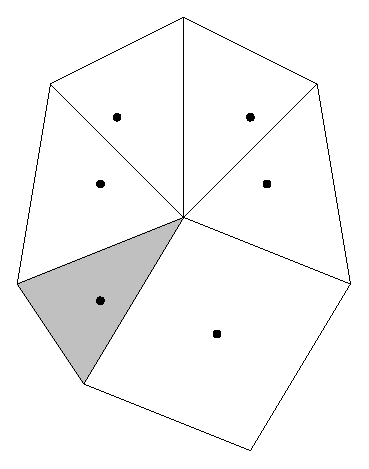
\includegraphics[width=.4\linewidth]{fig/volume_centrado.eps}
        \caption{Volume Centrado}
        \label{fig:volume_centrado}        
    \end{subfigure}
    \begin{subfigure}{.4\textwidth}
        \centering
        \includegraphics[width=.4\linewidth]{fig/volume_vertice.eps}
        \caption[]{Volume Baseado no vértice}
        \label{fig:volume_vertice}        
    \end{subfigure}

    \caption{Criação de Volumes de Controle}
    \label{fig:volume-controle}
  \end{figure}

\end{frame}


\section{Malhas não estruturadas}
\begin{frame}
  \frametitle{Malhas não estruturadas}
  Uma malha não estruturada pode ser considerada um caso limite de uma malha multiblocos na qual cada volume individual é tratado como um bloco.

  É o tipo de malha mais usada na indústria devido a sua capacidade de adaptação a qualquer tipo de problema. Normalmente são empregados triângulos ou quadriláteros para problemas bidimensionais.

  Cada bloco gerado pode ser denotado como volume de controle. Normalmente as variáveis de interesse para o problema são definidas no centróide desse elemento. Como na malha a seguir:

  \begin{figure}
    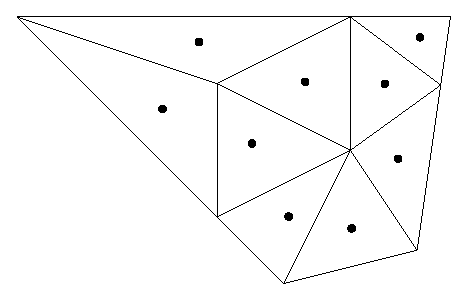
\includegraphics[width=0.4\linewidth]{variacao_suave.eps}
  \end{figure}

\end{frame}

\begin{frame}
  \frametitle{Malhas não estruturadas}

  \begin{block}{Qual a malha ideal?}
    Os elementos da malha devem ser o mais equiláteros o possível, ou seja, para uma malha triangular os angulos internos devem ser o mais próximo possível uns dos outros.
  \end{block}

  \begin{block}{Qual o motivo?}

    Isso permite que as funções de interpolação no métodos dos volumes finitos, representem bem as variáveis dentro do triângulo. Caso contrário observa-se uma elevada anisotropia nos coeficientes, o que reduz a taxa de convergência do processo de solução do sistema linear.

  \end{block}

\end{frame}
%------------------------------------------------
%------------------------------------------------
\section{Suavização de malhas não estruturadas}
\begin{frame}
  \frametitle{Suavização de malhas não estruturadas}
  Embora ferramentas de geração de malhas automáticas sejam amplamente usadas, essas ferramentas podem não garantir a qualidade das malhas. É possível que alguns elementos severamente distorcidos ou fora de forma sejam criados.

  \begin{figure}
    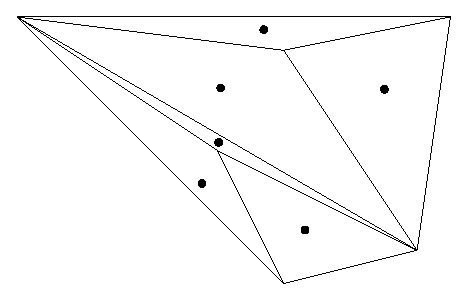
\includegraphics[width=0.4\linewidth]{variacao_brusca.eps}
  \end{figure}
\end{frame}

\begin{frame}
  \frametitle{Suavização de malhas não estruturadas}

  Existem várias maneiras de esquemas de suavização de malhas, tais como suavização Laplaciana e suavização baseada em otimização. Tipicamente cada método possui um compromisso entre qualidade e custo computacional. Por exemplo, a suavização Laplaciana requer um custo computacional muito baixo, mas frequentemente resulta em uma malha de baixa qualidade nos elementos ou mesmo com elementos inválidos. Por outro lado, enquanto suavizações baseados na otimização evitam elementos inválidos e obtém uma maior qualidade na malha, o custo computacional é muito maior que a suavização Laplaciana.

\end{frame}

\begin{frame}
  \frametitle{Suavização de malhas não estruturadas usando algoritmo genético.}

  Algoritmos Genéticos são métodos adaptativos que podem ser usados para resolver problemas envolvendo procura e otimização. Eles são baseados nos processos genéticos de organismos biológicos.

  O algoritmo genético pode evoluir soluções para problemas do mundo real, desde que tenham sido corretamente codificados.

  Usam uma analogia direta do mundo natural. Ele trabalha com uma população de indivíduos, cada um representando uma possível solução para um dado problema. Cada indivíduos recebe um nível de adaptabilidade de acordo com quão boa é a sua solução para o problema.

\end{frame}

\begin{frame}
  \frametitle{Suavização de malhas não estruturadas usando algoritmo genético}
  Os indivíduos altamente adaptados recebem uma maior oportunidade para reproduzir, por cruzamento com outro indivíduo na população. Isso produz novos indivíduos como descendentes, os quais compartilham algumas características de cada um dos seus pais. Os membros menos adaptados da população irão ter menor probabilidade de reprodução, de modo que eles desaparecem.
\end{frame}

\begin{frame}
  \frametitle{Método proposto}

  De modo a se utilizar do algoritmo genético para a suavização da malha, foi desenvolvido os seguintes passos:

  \begin{itemize}
    \item Geração de uma malha usando-se a triangulação de Delaunay
    \item Aplicação de uma distorção na malha.
    \item Desenvolvimento do algoritmo para suavizar essa malha.
  \end{itemize}
\end{frame}

\section{Triangulação de Delaunay}

\begin{frame}
  \frametitle{Triangulação de Delaunay}
  Imagine pontos aleatórios na tela.
  \begin{figure}
    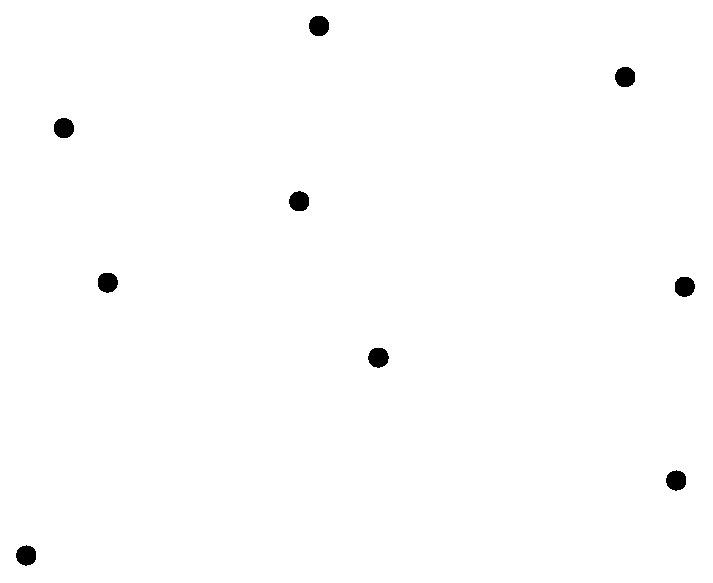
\includegraphics[width=0.5\linewidth]{dela1.eps}
  \end{figure}
\end{frame}

\begin{frame}
  \frametitle{Triangulação de Delaunay}
  Devemos criar uma malha triangular a partir desses pontos.
  \begin{figure}
    \includegraphics[width=0.5\linewidth]{dela2.eps}
  \end{figure}
\end{frame}

\begin{frame}
  \frametitle{Triangulação de Delaunay}

  \begin{block}{O que é?}
    É um processo para geração de triangulações a partir de um conjunto de pontos em um plano. Em tal triangulação nenhum ponto gerado está dentro do circuncírculo formado por qualquer triangulo.
  \end{block}

  \begin{block}{Porque é usado?}
    Ela otimiza simultaneamente os seguintes critérios:
    \begin{itemize}
      \item Maximização do mínimo ângulo interno dos triângulos
      \item Minimização do máximo circuncírculo das arestas
      \item Minimização do máximo mínimo cŕiculo de contenção das arestas
    \end{itemize}
  \end{block}
\end{frame}


\begin{frame}
  O circuncírculo de um triângulo é um círculo que passa por todos os seus vértices:

  \begin{figure}
    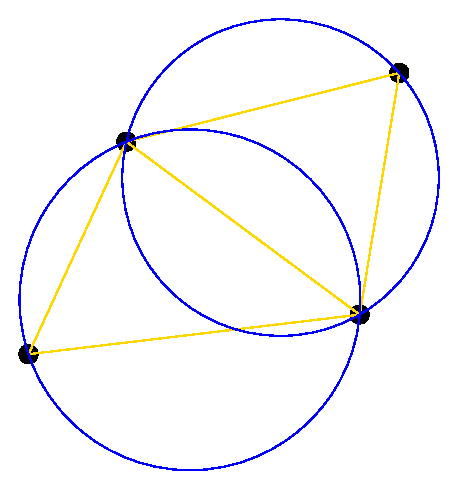
\includegraphics[width=0.3\linewidth]{dela3.eps}
  \end{figure}


\end{frame}


\begin{frame}
  \frametitle{Triangulação de Delaunay}

  Uma maneira de se criar uma triangulação de Delaunay é usando-se o algoritmo de Bowyer-Watson.

  Como exemplo temos os seguintes quatro vértices:

  \begin{figure}
    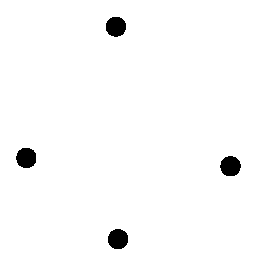
\includegraphics[width=0.3\linewidth]{dela4.eps}
  \end{figure}
\end{frame}


\begin{frame}
  \frametitle{Triangulação de Delaunay}

  Inicialmente, acha-se um triangulo contendo todos os pontos. Chamado de 'super-triangulo'


  \begin{figure}
    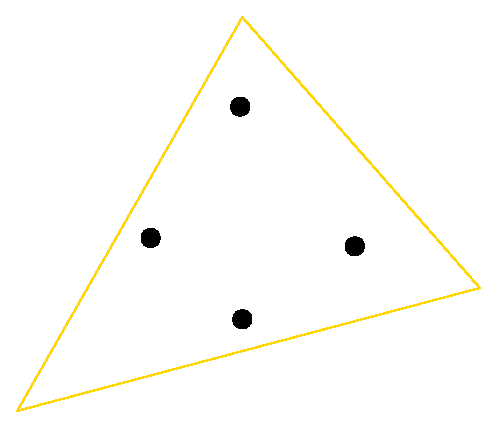
\includegraphics[width=0.5\linewidth]{dela5.eps}
  \end{figure}
\end{frame}

\begin{frame}
  \frametitle{Triangulação de Delaunay}

  Em seguida, seleciona-se um ponto qualquer e procura-se por triangulos cujo circuncirculo contenha esse ponto. Inicialmente tal triangulo é o super-triangulo.

  \begin{figure}
    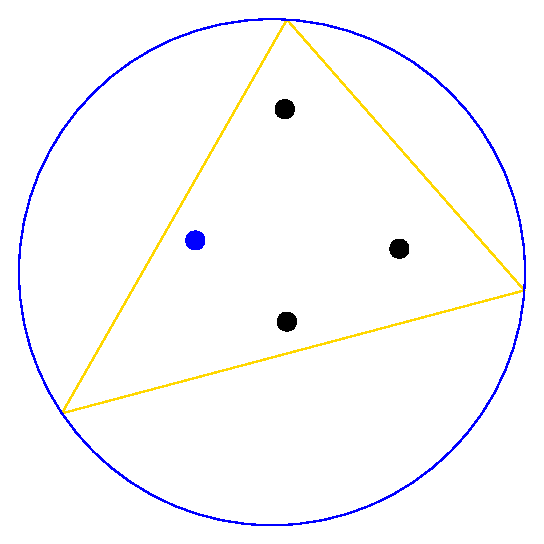
\includegraphics[width=0.5\linewidth]{dela6.eps}
  \end{figure}
\end{frame}

\begin{frame}
  \frametitle{Triangulação de Delaunay}

  Como o ponto está contido no circuncírculo, o triangulo não é um triangulo de Delaunay e portanto é descartado.

  A seguir o ponto é conectado com os vértices do triangulo de modo a se criar um novo conjunto de triangulos.

  \begin{figure}
    \includegraphics[width=0.5\linewidth]{dela7.eps}
  \end{figure}
\end{frame}

\begin{frame}
  \frametitle{Triangulação de Delaunay}

  Esse processo é repetido para todos os outros pontos:

  \begin{figure}
    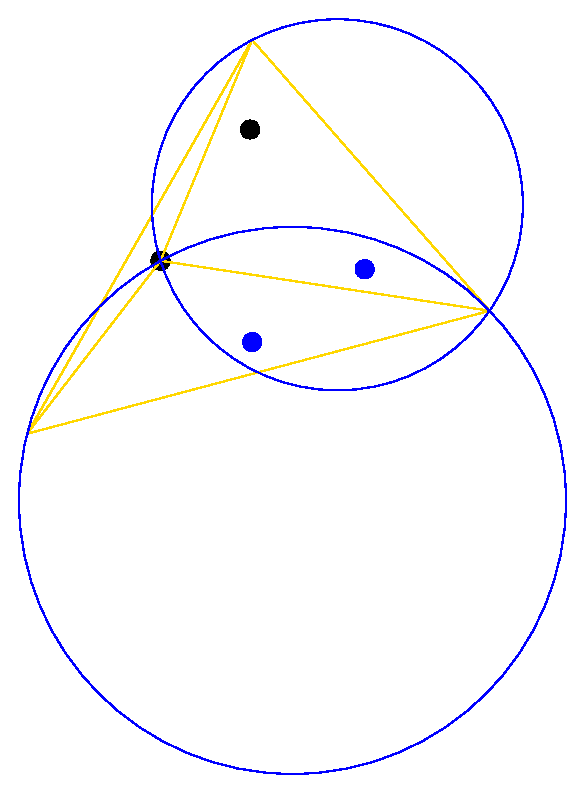
\includegraphics[width=0.5\linewidth]{dela8.eps}
  \end{figure}
\end{frame}

\begin{frame}
  \frametitle{Triangulação de Delaunay}

  Os dois pontos do passo anterior estão em circuncírculos logo seus triangulos são deletados:

  \begin{figure}
    \includegraphics[width=0.5\linewidth]{dela9.eps}
  \end{figure}
\end{frame}

\begin{frame}
  \frametitle{Triangulação de Delaunay}

  Seguindo o algorítmo, os pontos são conectados com os vértices dos triangulos apagados:

  \begin{figure}
    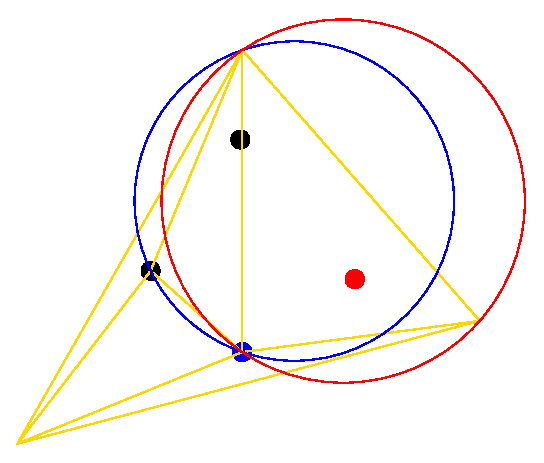
\includegraphics[width=0.5\linewidth]{dela10.eps}
  \end{figure}
  Percebe-se que apenas o ponto em vermelho está dentro de um circuncírculo, logo o triangulo deve ser apagado.
\end{frame}

\begin{frame}
  \frametitle{Triangulação de Delaunay}
  O resultado fica:

  \begin{figure}
    \includegraphics[width=0.5\linewidth]{dela11.eps}
  \end{figure}
\end{frame}

\begin{frame}
  \frametitle{Triangulação de Delaunay}
  Proceguindo com o altoritmo:

  \begin{figure}
    \includegraphics[width=0.5\linewidth]{dela12.eps}
  \end{figure}
\end{frame}

\begin{frame}
  \frametitle{Triangulação de Delaunay}
  Nesse ponto pode-se perceber que nenhum ponto está dentro de qualquer circuncírculo:

  \begin{figure}
    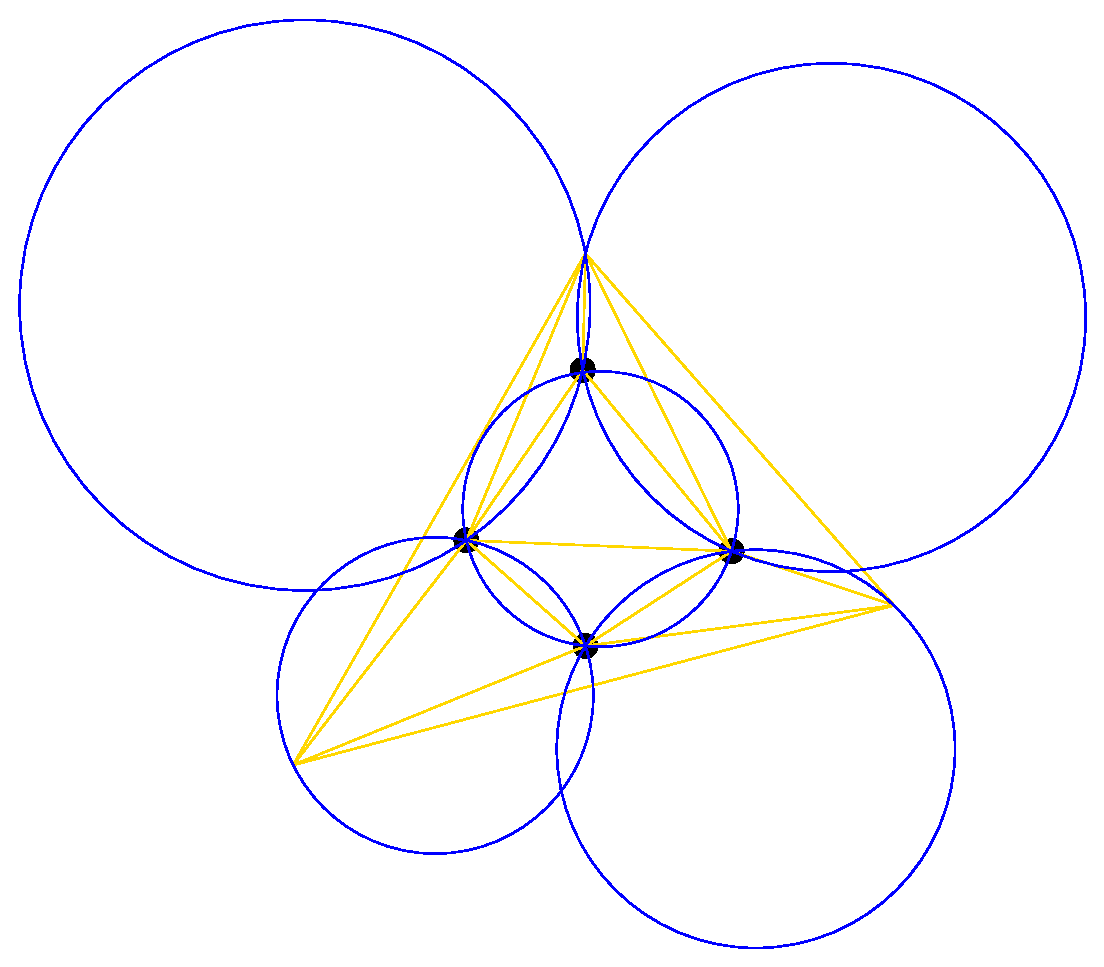
\includegraphics[width=0.8\linewidth]{dela13.eps}
  \end{figure}
\end{frame}

\begin{frame}
  \frametitle{Triangulação de Delaunay}
  Como último passo os vértices do super-triangulo são apagados assim como qualquer triangulo que os possua:

  \begin{figure}
    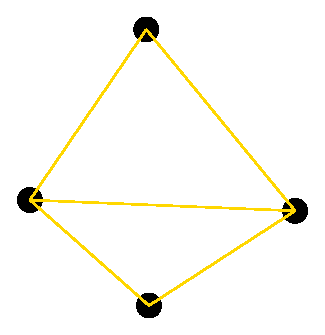
\includegraphics[width=0.3\linewidth]{dela14.eps}
  \end{figure}
\end{frame}

\section{Algoritmo de suavização}
\begin{frame}
  \frametitle{Algoritmo de suavização}

  O algorítmo tem como objetivo mover a posição de todos os nós internos da malha. Desse modo o algoritmo é aplicado sequencialmente a cada nó interno. Para cada nó é definido uma população de indivíduos cujo genótipo é um par de números, o primeiro para a posição da coordenada x e outro para a y. Tais membros são inicialmente gerados aleatoriamente. No total cada geração possui 300 indivíduos e é calculado 40 gerações.

\end{frame}

\begin{frame}
  \frametitle{Algoritmo de suavização}

  A função fitness, que irá determinar o quão apto a reprodução é um determinado nó(indivíduo) é calculada da seguinte forma:

  \begin{equation}
    SQ_i = \frac{4\sqrt{3}A_i}{\sum_{i=1}^3 l_i^2}
  \end{equation}

  Essa equação é calculada para todos os volumes que incluem o vértice e então somados, esse valor será maior quanto mais equilátero for o triangulo da malha. Desse modo cada indivíduo tem um genótipo definido como um par de valores (coordenadas x e y) e o seu fenótipo é dado por essa equação que define a média da qualidade dos volumes que compartilham esse vértice.
\end{frame}

\section{Resultados da pesquisa}
\begin{frame}
  \frametitle{Resultados da pesquisa}
  De modo a se conseguir comparar a performance do algoritmo genético na suavização da malha. Foi proposto um domínio em formato 'L':

  \begin{figure}
    \includegraphics[width=0.6\linewidth]{malha_inicial.png}
  \end{figure}
\end{frame}

\begin{frame}
  \frametitle{Malha distorcida}

  Essa malha gerada com a triangulação de Delaunay é então distorcida e é calculado os valores do maior e menor ângulo assim como a média e o desvio padrão dos ângulos das triangulações.

  Também foi calculado os valores da qualidade da malha conforme a equação que foi mostrada, mostrando o maior, menor, média e desvio padrão.

  \begin{figure}
    \includegraphics[width=0.6\linewidth]{malha-ruim.png}
  \end{figure}

\end{frame}

\begin{frame}
  \frametitle{Malha distorcida}

  \begin{table}[hb]
    \centering
    \par\caption{Ângulos da Malha Distorcida}
    \begin{tabular}{c|c|c|c}
      Maior      & menor    & média     & desvio padrão \\\hline\hline
      165.963757 & 6.340192 & 60.000000 & 30.017315     \\\hline
    \end{tabular}
    \label{tab:angulos-malha-distorcida}
  \end{table}

  \begin{table}[hb]
    \centering
    \par\caption{Qualidades da Malha Distorcida}
    \begin{tabular}{c|c|c|c}
      Maior    & menor    & média    & desvio padrão \\\hline\hline
      0.928007 & 0.029467 & 0.700351 & 0.227835      \\\hline
    \end{tabular}
    \label{tab:qualidades-malha-distorcida}
  \end{table}

\end{frame}

\begin{frame}
  \frametitle{Centroidal Path Tesselation}

  \begin{figure}
    \includegraphics[width=0.6\linewidth]{malha-cpt.png}
  \end{figure}

\end{frame}


\begin{frame}
  \frametitle{Centroidal Path Tesselation}

  \begin{table}[hb]
    \centering
    \par\caption{Ângulos da Malha CPT}
    \begin{tabular}{c|c|c|c}
      Maior      & menor     & média     & desvio padrão \\\hline\hline
      125.476562 & 18.434949 & 60.000000 & 16.412226     \\\hline
    \end{tabular}
    \label{tab:angulos-malha-cpt}
  \end{table}

  \begin{table}[hb]
    \centering
    \par\caption{Qualidades da Malha CPT}
    \begin{tabular}{c|c|c|c}
      Maior    & menor    & média    & desvio padrão \\\hline\hline
      0.997240 & 0.376030 & 0.889689 & 0.126673      \\\hline
    \end{tabular}
    \label{tab:qualidades-malha-cpt}
  \end{table}

\end{frame}

\begin{frame}
  \frametitle{Optimal Delaunay Tesselation}

  \begin{figure}
    \includegraphics[width=0.6\linewidth]{fig/malha-odt.png}
  \end{figure}

\end{frame}
\begin{frame}
  \frametitle{Optimal Delaunay Tesselation}

  \begin{table}[hb]
    \centering
    \par\caption{Ângulos da Malha ODT}
    \begin{tabular}{c|c|c|c}
      Maior      & menor     & média     & desvio padrão \\\hline\hline
      92.339656&36.765310&60.000000&14.499022\\\hline
    \end{tabular}
    \label{tab:angulos-malha-odt}
  \end{table}

  \begin{table}[hb]
    \centering
    \par\caption{Qualidades da Malha ODT}
    \begin{tabular}{c|c|c|c}
      Maior    & menor    & média    & desvio padrão \\\hline\hline
      0.997704&0.823047&0.926443&0.046574\\\hline
    \end{tabular}
    \label{tab:qualidades-malha-odt}
  \end{table}

\end{frame}

\begin{frame}
  \frametitle{Centroidal Voronoi Tesselation}

  \begin{figure}
    \includegraphics[width=0.6\linewidth]{fig/malha-cvt.png}
  \end{figure}

\end{frame}
\begin{frame}
  \frametitle{Centroidal Voronoi Tesselation}

  \begin{table}[hb]
    \centering
    \par\caption{Ângulos da Malha CVT}
    \begin{tabular}{c|c|c|c}
      Maior      & menor     & média     & desvio padrão \\\hline\hline
      98.568632&36.794950	&60.000000&17.275253\\\hline
    \end{tabular}
    \label{tab:angulos-malha-cvt}
  \end{table}

  \begin{table}[hb]
    \centering
    \par\caption{Qualidades da Malha CVT}
    \begin{tabular}{c|c|c|c}
      Maior    & menor    & média    & desvio padrão \\\hline\hline
      0.990750&0.787629&0.907101&0.059118\\\hline
    \end{tabular}
    \label{tab:qualidades-malha-cvt}
  \end{table}

\end{frame}

\begin{frame}
  \frametitle{Angle Based Tesselation}

  \begin{figure}
    \includegraphics[width=0.6\linewidth]{fig/malha-angulos.png}
  \end{figure}

\end{frame}
\begin{frame}
  \frametitle{Angle Based Tesselation}

  \begin{table}[hb]
    \centering
    \par\caption{Ângulos da Malha Ângulos}
    \begin{tabular}{c|c|c|c}
      Maior      & menor     & média     & desvio padrão \\\hline\hline
      90.003446	&44.996564&60.000000&21.268508\\\hline
    \end{tabular}
    \label{tab:angulos-malha-angulos}
  \end{table}

  \begin{table}[hb]
    \centering
    \par\caption{Qualidades da Malha Ângulos}
    \begin{tabular}{c|c|c|c}
      Maior    & menor    & média    & desvio padrão \\\hline\hline
      0.866070&0.865999&0.866027	&0.000013\\\hline
    \end{tabular}
    \label{tab:qualidades-malha-angulos}
  \end{table}

\end{frame}

\begin{frame}
  \frametitle{Gurobi Optimization Based Tesselation}

  Para a otimização usando-se o Gurobi, foi definido como função objetivo a ser minimizada a distância total dos nós internos para os nós vizinhos.

  \begin{figure}
    \includegraphics[width=0.6\linewidth]{fig/malha-gurobi.png}
  \end{figure}

\end{frame}
\begin{frame}
  \frametitle{Gurobi Optimization Based Tesselation}

  \begin{table}[hb]
    \centering
    \par\caption{Ângulos da Malha Gurobi}
    \begin{tabular}{c|c|c|c}
      Maior      & menor     & média     & desvio padrão \\\hline\hline
      118.072487	&30.541971&60.000000&24.045397\\\hline
    \end{tabular}
    \label{tab:angulos-malha-gurobi}
  \end{table}

  \begin{table}[hb]
    \centering
    \par\caption{Qualidades da Malha Gurobi}
    \begin{tabular}{c|c|c|c}
      Maior    & menor    & média    & desvio padrão \\\hline\hline
      0.977771&0.618590&0.831586&0.098368\\\hline
    \end{tabular}
    \label{tab:qualidades-malha-gurobi}
  \end{table}

\end{frame}

\begin{frame}
  \frametitle{Genetic Algorithm Based Tesselation}

  \begin{figure}
    \includegraphics[width=0.6\linewidth]{fig/malha-ga.png}
  \end{figure}

\end{frame}
\begin{frame}
  \frametitle{Genetic Algorithm Based Tesselation}
  \begin{table}[hb]
    \centering
    \par\caption{Ângulos da Malha GA}
    \begin{tabular}{c|c|c|c}
      Maior      & menor     & média     & desvio padrão \\\hline\hline
      103.651693&36.916308&60.000000&21.561762\\\hline
    \end{tabular}
    \label{tab:angulos-malha-ga}
  \end{table}

  \begin{table}[hb]
    \centering
    \par\caption{Qualidades da Malha GA}
    \begin{tabular}{c|c|c|c}
      Maior    & menor    & média    & desvio padrão \\\hline\hline
      0.924401&0.751680&0.862425&0.033582\\\hline
    \end{tabular}
    \label{tab:qualidades-malha-ga}
  \end{table}
\end{frame}

\begin{frame}
  \frametitle{Comparação entre os métodos}

  Na tabela \ref{tab:comparacao-analitico} está o valor da média das diferenças entre o valor analítico e numérico para todos os algorítmos usados no trabalho em ordem crescente, ou seja, por essa métrica o algorítmo de melhoramento por ângulos e o genético foram os melhores.

\begin{table}
    \centering
    \par\caption{Comparação entre as médias das diferenças em relação ao valor analítico}
    \begin{tabular}{c|c}
        Algoritmo&diferença\\\hline\hline
        Ângulos  &  0.054529 \\\hline
        Genético &  0.054563 \\\hline
        Gurobi   &  0.056215 \\\hline
        CPT      &  0.060670 \\\hline
        ODT      &  0.060929 \\\hline
        CVT      &  0.062826 \\\hline
    \end{tabular}
    \label{tab:comparacao-analitico}
\end{table}

\end{frame}

\begin{frame}
  \frametitle{Comparação entre os métodos}

  Já na tabela \ref{tab:comparacao-qualidade} temos a métrica da média das qualidades conforme foi definido. Nesse caso o melhor algoritmo foi o ODT.

\begin{table}
    \centering
    \par\caption{Comparação entre as médias qualidades dos volumes de controle}
    \begin{tabular}{c|c}
        Algoritmo&diferença\\\hline\hline
        ODT      &  0.926443 \\\hline
        CPT      &  0.919103 \\\hline
        CVT      &  0.907101 \\\hline
        Ângulos  &  0.866027 \\\hline
        Genético &  0.860447 \\\hline
        Gurobi   &  0.831586 \\\hline
    \end{tabular}
    \label{tab:comparacao-qualidade}
\end{table}

\end{frame}

\section{Conclusão}
\begin{frame}
  \frametitle{Conclusão}
  O trabalho aborda a importância da suavização de uma malha não estruturada para minimizar os erros das aproximações com o método dos volumes finitos e compara vários métodos diferentes.

  O algoritmo genético é implementado mostrando que ele melhora a malha inicial, mesmo assim percebe-se um custo computacional mais elevado em relação a outros métodos.
\end{frame}

\end{document}